\documentclass[a4paper,11pt]{article}
\usepackage{sbpo-template}
\usepackage[brazil]{babel}
\usepackage[utf8]{inputenc}
\usepackage[T1]{fontenc}
\usepackage{amsmath,amssymb}
\usepackage{url}
\usepackage[square]{natbib}
\usepackage{indentfirst}
\usepackage{fancyhdr}
\usepackage{graphicx}
\usepackage{booktabs}
\usepackage{tabularx}
\usepackage{xcolor}
\usepackage[colorlinks=true, linkcolor=blue, citecolor=blue, urlcolor=blue]{hyperref}



\pagestyle{fancy}
\fancyhf{}
\fancyhead[C]{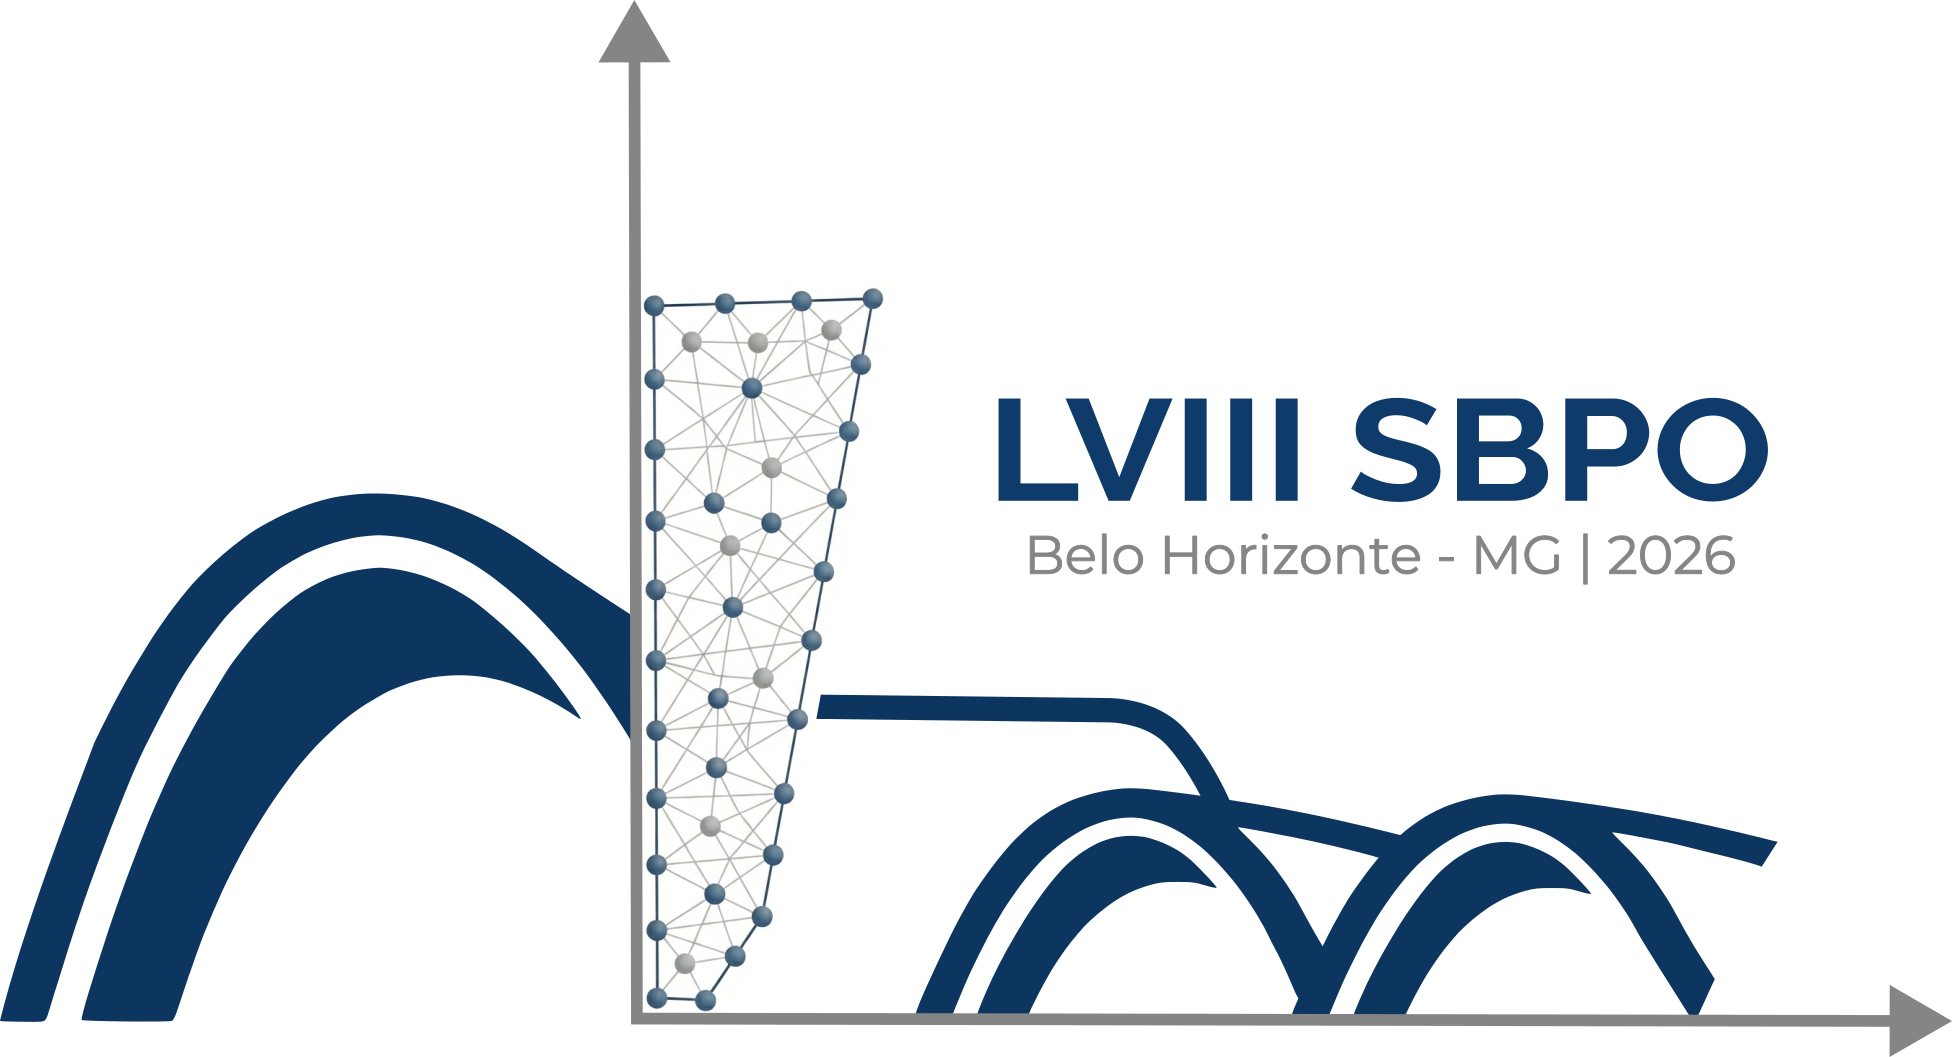
\includegraphics[scale=0.5]{sbpo2026-header-logo.png}}
\renewcommand{\headruleskip}{-1mm}
\setlength\headheight{86pt}
\addtolength{\textheight}{-86pt}
\setlength{\headsep}{5mm}
\setlength{\footskip}{4.08003pt}

\begin{document}

\title{Dashboard Interativo para o Ensino de Planejamento Agregado da Produção:\\
uma Ferramenta \textit{Open-Source} Baseada em Streamlit}

\maketitle
\thispagestyle{fancy}

\author{
\name{Leonardo Costa}
\institute{Departamento de Engenharia de Produção -- Universidade Federal Fluminense}
\iaddress{Rua Passo da Pátria 156, Niterói -- RJ, CEP 24210-240}
\email{leo\_costa@id.uff.br}
}


\author{
\name{Helder G. Costa}
\institute{Departamento de Engenharia de Produção -- Universidade Federal Fluminense}
\iaddress{Rua Passo da Pátria 156, Niterói -- RJ, CEP 24210-240}
\email{heldergc@id.uff.br}
}


\vspace{8mm}
\begin{resumo}
Este artigo apresenta um \textit{dashboard} interativo \textit{open-source} para o apoio ao  ensino das técnicas e conceitos de  Planejamento Agregado da Produção (PAP). Desenvolvido Python com as bibliotecas Streamlit, Plotly e SciPy. A ferramenta integra, em uma única interface reativa, seis métodos clássicos de PAP: Estratégia de Acompanhamento da Demanda, Produção Nivelada, Estratégia Mista, Programação Linear (PL), Método do Transporte e Tentativa-e-Erro. Adicionalmente, incorpora extensões modernas como variáveis inteiras via Programação Linear Inteira Mista
(PLIM) e três políticas de escassez (pedidos em atraso, sem escassez e venda perdida).
Um estudo de caso com horizonte de 12 períodos demonstra o uso comparativo dos métodos,
evidenciando que a PL obtém o menor custo total. A ferramenta está disponível publicamente no Streamlit Cloud, podendo ser utilizada sem instalação.
\end{resumo}

\bigskip
\begin{palchaves}
Planejamento agregado da produção. Ferramenta educacional. Programação linear. Dashboard interativo. 

\bigskip
\noindent{Tópicos (em ordem de prioridade):
1. Ensino de Pesquisa Operacional.
2. Planejamento da Produção / \textit{Supply Chain}.}
\end{palchaves}

\vspace{8mm}

\begin{abstract}
This paper presents an open-source interactive dashboard for teaching Aggregate Production
Planning (APP), developed in Python using the Streamlit, Plotly and SciPy libraries.
The tool integrates six classical APP methods in a single reactive web interface:
Chase Demand Strategy, Level Production, Mixed/Hybrid Strategy, Linear Programming (LP),
Transportation Method and Trial-and-Error. It further incorporates modern extensions such
as integer variables via Mixed-Integer Linear Programming (MILP) and three shortage
policies (backorders, no-shortages and lost sales). A twelve-period case study demonstrates
the comparative use of the methods, showing that LP achieves the lowest total cost.
The tool is publicly available on GitHub and Streamlit Cloud and requires no installation.
\end{abstract}

\bigskip
\begin{keywords}
Aggregate production planning. Educational tool. Linear programming. Interactive dashboard. Open-source.

\bigskip
\noindent{Paper topics (in order of priority):
1. Teaching Operations Research.
2. Production Planning / Supply Chain.}
\end{keywords}


\newpage

% ─────────────────────────────────────────────────────────────────────────────
\section{Introdução}
% ─────────────────────────────────────────────────────────────────────────────

O Planejamento Agregado da Produção (PAP) é um tema central nos cursos de Engenharia de
Produção e Administração, situando-se no nível tático do planejamento hierárquico de
sistemas de produção e distribuição~\citep{chase2006,heizer2017}. Seu objetivo é
determinar, para um horizonte de médio prazo (tipicamente de 3 a 18 meses), os níveis
ótimos de produção, mão-de-obra, estoques, horas extras e subcontratação, de forma a
minimizar o custo total enquanto atende à demanda prevista dentro das restrições de
capacidade.

Apesar de sua importância, o ensino do PAP enfrenta desafios práticos. As ferramentas
disponíveis costumam ser planilhas estáticas que exigem reconfiguração manual, softwares comerciais com custo de licenciamento elevado ou implementações acadêmicas isoladas que
cobrem apenas um método por vez. A ausência de uma plataforma que integre múltiplos
métodos de forma comparativa e interativa dificulta que o aluno desenvolva a intuição
sobre os \textit{trade-offs} entre as diferentes estratégias.

Este trabalho apresenta o \textbf{Aggregate Planning Dashboard}, um \textit{dashboard}
interativo \textit{open-source} desenvolvido em Python, que integra seis métodos
clássicos de PAP em uma única interface web reativa. As principais contribuições são:
(i)~integração inédita de seis métodos de PAP, incluindo heurísticas e a solução ótima
por PL/PLIM, em uma interface comparativa unificada; (ii)~extensão a variáveis inteiras
via PLIM (\texttt{scipy.optimize.milp}); (iii)~modelagem de três políticas de tratamento
de escassez de demanda; (iv)~guia teórico integrado, disponível para download e uso
\textit{offline}; e (v)~implantação gratuita em nuvem (Streamlit Cloud), acessível sem
instalação.

O artigo está organizado da seguinte forma: a Seção~\ref{sec:pap} revisita brevemente o
problema de PAP; a Seção~\ref{sec:ferramenta} descreve a ferramenta; a
Seção~\ref{sec:modelos} apresenta os modelos e métodos implementados; a
Seção~\ref{sec:caso} traz o estudo de caso ilustrativo; e a Seção~\ref{sec:conclusao}
encerra com as conclusões e trabalhos futuros.


% ─────────────────────────────────────────────────────────────────────────────
\section{Planejamento Agregado da Produção}
\label{sec:pap}
% ─────────────────────────────────────────────────────────────────────────────

O PAP busca determinar, para cada período $t = 1,\ldots,T$ de um horizonte de
planejamento, os valores das principais variáveis de decisão:
$W_t$ (nível de mão-de-obra), $P_t$ (produção regular), $H_t$ e $F_t$ (contratações e
demissões), $I_t$ (estoque final), $O_t$ (horas extras) e $S_t$ (subcontratação).
A função objetivo genérica minimiza o custo total:
%
\begin{equation}
  \label{eq:custo}
  Z = \sum_{t=1}^{T}\bigl(
    c_{RT}\,P_t + c_H\,H_t + c_F\,F_t + c_e\,I_t^{+} + c_B\,I_t^{-}
    + c_{OT}\,O_t + c_S\,S_t
  \bigr),
\end{equation}
%
onde $c_{RT}$, $c_H$, $c_F$, $c_e$, $c_B$, $c_{OT}$ e $c_S$ são os custos unitários
de produção regular, contratação, demissão, estoque, pedido em atraso, hora extra e
subcontratação, respectivamente; $I_t^{+} = \max(I_t,0)$ representa estoque positivo e
$I_t^{-} = \max(-I_t,0)$ representa \textit{backorder}.

As principais restrições modelam o balanço de estoque
($I_t = I_{t-1} + P_t + O_t + S_t - D_t$),
o balanço de mão-de-obra ($W_t = W_{t-1} + H_t - F_t$),
a relação entre produção e mão-de-obra ($P_t \leq \phi\,W_t$, onde $\phi$ é a
produtividade em unidades por trabalhador por período),
e os limites de capacidade~\citep{hanssmann1960,silver1967}.

A literatura clássica propõe abordagens que vão desde as heurísticas simples de
Acompanhamento da Demanda (\textit{Chase}) e Produção Nivelada (\textit{Level}), passando
pelo Método do Transporte de~\citet{bowman1956} e a regra de decisão linear de
\citet{holt1955}, até formulações de programação matemática. Para uma revisão abrangente,
veja \citet{arenales2015} e \citet{krajewski2013}.

\subsection{Revisão da Literatura sobre Modelagem do PAP}

O Quadro~\ref{tab:lit} sintetiza trabalhos representativos sobre a modelagem do PAP,
agrupados cronologicamente desde os modelos fundacionais até abordagens contemporâneas de
programação matemática avançada. A análise evidencia três tendências dominantes:
(i)~a transição dos modelos analíticos e heurísticos clássicos para formulações de
Programação Linear (PL) e Programação Linear Inteira Mista (PLIM); (ii)~a incorporação
crescente de incerteza via lógica fuzzy e programação por metas; e (iii)~a carência de
ferramentas educacionais que integrem múltiplos métodos de forma comparativa e interativa.
Em particular, nenhum dos trabalhos revisados propõe simultaneamente a modelagem de
políticas de escassez distintas e uma interface pedagógica dedicada, lacuna que o presente
trabalho se propõe a preencher.

\begin{table}[htbp]
\centering
\caption{Síntese de trabalhos representativos sobre modelagem do PAP.}
\label{tab:lit}
\begin{tabularx}{\textwidth}{@{}p{3.1cm}p{3.0cm}p{2.0cm}p{1.4cm}p{1.4cm}X@{}}
\toprule
\textbf{Referência} &
\textbf{Abordagem} &
\textbf{Variáveis} &
\textbf{Pol.\ escassez} &
\textbf{Foco} &
\textbf{Ferramenta} \\
\midrule
\citet{holt1955}       & Regra de decisão linear quadrática (HMMS) & P, W, H, F, I & Não & Teórico & Analítico \\
\citet{bowman1956}     & Método do Transporte (PL) & P, I & Não & Teórico & PL manual \\
\citet{hanssmann1960}  & Programação Linear & P, W, O, S, I & Não & Teórico & PL \\
\citet{silver1967}     & Suavização de produção e força de trabalho & P, W, H, F, I & Não & Teórico & Analítico \\
\citet{nam1992}        & Survey de modelos e metodologias & Variadas & Variado & Survey & -- \\
\citet{wang2004}       & PL fuzzy multi-objetivo & P, W, O, S, I & Não & Aplicado & Fuzzy LP \\
\citet{leung2009}      & Programação por metas & P, W, O, S, I & Sim & Aplicado & Goal prog. \\
\citet{jamalnia2009}   & Goal programming fuzzy híbrido & P, W, O, S, I & Não & Aplicado & Fuzzy GP \\
\citet{baykasoglu2010} & Programação matemática fuzzy & P, W, O, S, I & Não & Aplicado & MOLP \\
\citet{ramezanian2012} & PLIM + metaheurísticas & P, W, O, S, I & Não & Aplicado & MILP + GA \\
\textbf{Este trabalho} & \textbf{PL/PLIM + heurísticas} & \textbf{P, W, H, F,} \textbf{O, S, I, B, L} & \textbf{3 políticas} & \textbf{Educacional} & \textbf{Dashboard web} \\
\bottomrule
\end{tabularx}
\smallskip
\footnotesize
\textit{Legenda -- Variáveis}: P: produção; W: mão-de-obra; H/F: contratação/demissão;
O: horas extras; S: subcontratação; I: estoque; B: \textit{backorder}; L: venda perdida.\\
\textit{Pol.\ escassez}: política de tratamento de demanda não atendida.
\end{table}


% ─────────────────────────────────────────────────────────────────────────────
\section{A Ferramenta Desenvolvida}
\label{sec:ferramenta}
% ─────────────────────────────────────────────────────────────────────────────

\subsection{Arquitetura e Tecnologias}

O \textit{dashboard} foi desenvolvido inteiramente em Python~3, com código aberto sob
licença MIT. A arquitetura é composta por dois módulos principais:

\begin{itemize}
  \item \texttt{solvers.py}: módulo de cálculo puro, sem dependências de interface.
    Implementa as seis estratégias de PAP e a função utilitária \texttt{compare\_all}.
  \item \texttt{app.py}: módulo de interface, que define o \textit{layout} do
    \textit{dashboard} com Streamlit e chama \texttt{solvers.py} de forma reativa.
\end{itemize}

As bibliotecas utilizadas são: \textbf{Streamlit}~\citep{streamlit2024} para a interface
web reativa; \textbf{Plotly}~\citep{plotly2024} para visualizações interativas;
\textbf{SciPy}~\citep{scipy2020} para os solvers de otimização
(\texttt{linprog} e \texttt{milp}); \textbf{NumPy} e \textbf{Pandas} para manipulação
numérica e tabular.

O repositório está disponível em \url{https://github.com/helderhgc/aggregate_planing}
e o aplicativo pode ser acessado diretamente no navegador, sem instalação, pelo
Streamlit Cloud~\citep{github2026}.

\subsection{Funcionalidades Principais}

A Figura~\ref{fig:dashboard} ilustra a interface principal do \textit{dashboard}.
O painel lateral (\textit{sidebar}) centraliza todos os parâmetros de entrada:

\begin{itemize}
  \item \textbf{Demanda}: entrada manual por período, carregamento de arquivo CSV/Excel
    ou seleção de cenários pré-definidos (\textit{Alta Sazonalidade},
    \textit{Demanda Estável} e \textit{Pico de Demanda}). A troca de cenário atualiza
    instantaneamente todos os campos e resultados.
  \item \textbf{Parâmetros de custo e capacidade}: sete componentes de custo,
    máximo de mão-de-obra, fração máxima de horas extras e limite de subcontratação.
  \item \textbf{Condições iniciais}: estoque e nível de mão-de-obra no período~0.
  \item \textbf{Tipo de variáveis}: opções para forçar variáveis inteiras de mão-de-obra
    e/ou produção (ativa a formulação PLIM).
  \item \textbf{Política de escassez}: seleção entre pedidos em atraso
    (\textit{backorders}), sem escassez e venda perdida (\textit{lost sales}).
\end{itemize}

A área principal apresenta, de forma automática e reativa: cartões de KPIs (custo total,
contratações, demissões, estoque médio, horas extras); e sete abas temáticas -- Previsão
de Demanda, Tabela do Plano, Produção \& Estoque, Dinâmica de Mão-de-Obra, Detalhamento
de Custos, Comparação de Estratégias e Guia Teórico. As abas de Preços-Sombra (LP)
e Tableau do Transporte aparecem condicionalmente conforme a estratégia selecionada.

\begin{figure}[htbp]
  \centering
  % Substitua pelo screenshot real do dashboard
  \fbox{\parbox{0.92\textwidth}{\centering\vspace{2cm}
  [Inserir screenshot do dashboard -- painel lateral + gráfico de produção]
  \vspace{2cm}}}
  \caption{Interface principal do Aggregate Planning Dashboard. À esquerda, o painel de
  parâmetros; à direita, os KPIs e o gráfico de mix de produção (empilhado) com a curva
  de demanda sobreposta.}
  \label{fig:dashboard}
\end{figure}

\subsection{Guia Teórico Integrado}

A ferramenta inclui um guia teórico completo em formato HTML (\texttt{theory.html}),
diretamente acessível na aba~\textit{Theory} do \textit{dashboard} e disponível para
download e uso \textit{offline}. O guia cobre todos os métodos implementados, com
formulações matemáticas, exemplos numéricos resolvidos e a seção de análise de
sensibilidade via preços-sombra. Essa característica é especialmente relevante para o
contexto pedagógico, pois permite que o estudante consulte a teoria enquanto manipula o
modelo interativamente.

\subsection{Posicionamento em Relação a Ferramentas Existentes}

O Quadro~\ref{tab:ferramentas} compara o \textit{Aggregate Planning Dashboard} com as
principais alternativas disponíveis para ensino e análise de PAP. Os critérios adotados
abrangem aspectos de acessibilidade, cobertura metodológica e adequação pedagógica.

\begin{table}[htbp]
\centering
\caption{Comparação entre ferramentas para ensino e análise do PAP.}
\label{tab:ferramentas}
\resizebox{\textwidth}{!}{%
\begin{tabular}{@{}p{3.0cm}p{1.5cm}p{1.7cm}p{1.7cm}p{1.1cm}p{1.7cm}p{1.5cm}p{1.9cm}p{1.5cm}@{}}
\toprule
\textbf{Ferramenta} &
\textbf{Cód.\ aberto} &
\textbf{Web / s/ instal.} &
\textbf{Métodos PAP} &
\textbf{PLIM} &
\textbf{Pol.\ escassez} &
\textbf{Vis.\ interativa} &
\textbf{Comparação integrada} &
\textbf{Guia teórico} \\
\midrule
POM-QM~\citep{weiss2016}
  & Não & Não & 3 básicos & Não & Não & Limitada & Não & Não \\
Excel + Solver
  & Não & Não & Manual & Parcial & Manual & Estática & Não & Não \\
LINGO/LINDO
  & Não & Não & Geral & Sim & Manual & Não & Não & Não \\
Pyomo~\citep{bynum2021}
  & Sim & Não & Geral & Sim & Manual & Não & Não & Não \\
\textbf{Este trabalho}
  & \textbf{Sim} & \textbf{Sim} & \textbf{6 métodos} & \textbf{Sim} & \textbf{3 políticas} & \textbf{Sim} & \textbf{Sim} & \textbf{Sim} \\
\bottomrule
\end{tabular}%
}
\par\smallskip
{\footnotesize
\textit{Legenda -- Cód.\ aberto}: disponibilidade do código-fonte;
\textit{Web/s/ instal.}: acesso via navegador sem instalação local;
\textit{Métodos PAP}: estratégias de PAP implementadas nativamente;
\textit{PLIM}: suporte a variáveis inteiras;
\textit{Pol.\ escassez}: políticas de demanda não atendida;
\textit{Vis.\ interativa}: gráficos dinâmicos em tempo real;
\textit{Comparação integrada}: painel comparativo automático entre métodos;
\textit{Guia teórico}: material didático embutido na interface.}
\end{table}

A análise evidencia que nenhuma das ferramentas existentes reúne simultaneamente os
atributos de código aberto, acesso \textit{web} sem instalação, cobertura de seis métodos,
suporte a PLIM, múltiplas políticas de escassez e interface comparativa com guia teórico
integrado. O \textit{Aggregate Planning Dashboard} é a única solução que combina todos
esses atributos, ocupando um nicho específico voltado ao ensino de PAP de forma integrada
e acessível.


% ─────────────────────────────────────────────────────────────────────────────
\section{Modelos e Métodos Implementados}
\label{sec:modelos}
% ─────────────────────────────────────────────────────────────────────────────

\subsection{Estratégias Heurísticas}

\textbf{Acompanhamento da Demanda (\textit{Chase Demand}):} a produção de cada período
iguala a demanda ($P_t = D_t$); a mão-de-obra é ajustada conseqüentemente. Tende a
minimizar estoques ao custo de elevada rotatividade de mão-de-obra.

\textbf{Produção Nivelada (\textit{Level Production}):} a força de trabalho e a taxa
de produção são mantidas constantes ao longo do horizonte, com ajuste inicial mínimo.
O estoque absorve a variação sazonal. Minimiza custos de contratação/demissão em troca
de maior custo de estocagem.

\textbf{Estratégia Mista (\textit{Mixed/Hybrid}):} combina estabilidade de mão-de-obra
com flexibilidade operacional. A partir de um nível nivelado, horas extras e
subcontratação preenchem eventuais déficits de capacidade, observando os limites de
capacidade configurados pelo usuário.

As três heurísticas suportam as opções de arredondamento para variáveis inteiras e as
três políticas de escassez.

\subsection{Modelo de Programação Linear}

O modelo de PL é formulado com $9T$ variáveis de decisão, organizadas em fatias:
produção regular $P_t$, horas extras $O_t$, subcontratação $S_t$, mão-de-obra $W_t$,
nível de produção total $R_t$, contratações $H_t$ e demissões $F_t$,
pedidos em atraso $I_t^{-}$ e vendas perdidas $L_t$.
A função objetivo minimiza o custo total conforme a Equação~(\ref{eq:custo}).
As restrições incluem o balanço de estoque, o balanço de mão-de-obra, os limites de
capacidade e as condições de não-negatividade.

A implementação utiliza \texttt{scipy.optimize.linprog} para o caso contínuo e
\texttt{scipy.optimize.milp}~\citep{scipy2020} quando variáveis inteiras são ativadas,
por meio de um vetor de integralidade. Após a resolução do modelo contínuo, os
\textbf{preços-sombra} (valores duais) das restrições de balanço de estoque e de
mão-de-obra são extraídos e exibidos na aba dedicada do \textit{dashboard}, permitindo
análise de sensibilidade diretamente na interface.

\subsection{Método do Transporte}

O PAP é reformulado como um problema de transporte clássico~\citep{bowman1956}, em que
as fontes representam modalidades de produção (por período: tempo regular, hora extra e
subcontratação) e os destinos representam os períodos de demanda. O custo de alocação
de uma unidade produzida no período~$i$ e entregue no período~$j$ ($j \geq i$) incorpora
o custo de produção mais o custo de estocagem acumulado pelos $(j-i)$ períodos de atraso.
A solução ótima do problema de transporte é obtida por PL (ou PLIM quando inteiros são
solicitados), e o \textit{tableau} completo -- com alocações e custos unitários por
célula -- é exibido em aba dedicada.

\subsection{Método Tentativa-e-Erro}

Nesta modalidade, o usuário define manualmente, período a período, os valores de
produção, mão-de-obra, horas extras e subcontratação por meio de uma tabela editável.
O sistema verifica a viabilidade do plano e calcula imediatamente o custo total resultante.
É uma estratégia didaticamente valiosa, pois incentiva o aluno a raciocinar sobre as
implicações de cada decisão individual~\citep{heizer2017}.

\subsection{Políticas de Escassez e Variáveis Inteiras}

A ferramenta suporta três políticas para demanda não atendida:
(i)~\textbf{Pedidos em atraso} (\textit{backorders}): estoque negativo é permitido com
custo $c_B$ por unidade por período; (ii)~\textbf{Sem escassez}: estoque negativo é
proibido por restrição, podendo tornar o problema inviável; e
(iii)~\textbf{Venda perdida} (\textit{lost sales}): demanda não atendida é descartada
com custo de oportunidade $c_{LS}$ por unidade, modelada pela variável $L_t \geq 0$
adicionada ao balanço de estoque.

Quando ativada, a opção de \textbf{variáveis inteiras} força $W_t, H_t, F_t \in
\mathbb{Z}_{\geq 0}$ (mão-de-obra inteira) e/ou $P_t, O_t, S_t \in \mathbb{Z}_{\geq 0}$
(produção inteira), ativando automaticamente a formulação PLIM.


% ─────────────────────────────────────────────────────────────────────────────
\section{Estudo de Caso Ilustrativo}
\label{sec:caso}
% ─────────────────────────────────────────────────────────────────────────────

\subsection{Dados do Cenário}

O cenário-padrão da ferramenta corresponde a uma empresa com planejamento mensal em
horizonte de 12 períodos (janeiro a dezembro), com demanda de caráter sazonal. Os dados
de entrada estão resumidos na Tabela~\ref{tab:dados}.

\begin{table}[htbp]
\centering
\caption{Parâmetros do cenário-padrão.}
\label{tab:dados}
\begin{tabular}{@{}lrl@{}}
\toprule
\textbf{Parâmetro} & \textbf{Valor} & \textbf{Unidade} \\
\midrule
Estoque inicial & 100 & unidades \\
Mão-de-obra inicial & 40 & trabalhadores \\
Produtividade ($\phi$) & 15 & unid./trabalhador/período \\
Mão-de-obra máxima & 80 & trabalhadores \\
Máx. horas extras & 25\% & da prod. regular \\
Máx. subcontratação & 200 & unidades/período \\
\midrule
Custo tempo regular ($c_{RT}$) & 1.200 & R\$/unidade \\
Custo de contratação ($c_H$) & 800 & R\$/trabalhador \\
Custo de demissão ($c_F$) & 1.500 & R\$/trabalhador \\
Custo de estoque ($c_e$) & 50 & R\$/unidade/período \\
Custo de atraso ($c_B$) & 90 & R\$/unidade/período \\
Custo de hora extra ($c_{OT}$) & 1.800 & R\$/unidade \\
Custo de subcontratação ($c_S$) & 2.000 & R\$/unidade \\
\bottomrule
\end{tabular}
\begin{tabular}{@{}ccccccccccccc@{}}
\toprule
\textbf{Período} & Jan & Fev & Mar & Abr & Mai & Jun & Jul & Ago & Set & Out & Nov & Dez \\
\midrule
\textbf{Demanda} & 420 & 390 & 450 & 510 & 580 & 650 & 700 & 670 & 580 & 500 & 450 & 380 \\
\bottomrule
\end{tabular}
\end{table}

\subsection{Comparação das Estratégias}

A Tabela~\ref{tab:comparacao} apresenta os resultados obtidos pelas cinco estratégias automaticamente comparadas pelo \textit{dashboard}, adotando a política de pedidos em atraso (\textit{backorders}) e variáveis contínuas.

\begin{table}[htbp]
\centering
\caption{Comparação das estratégias de PAP -- cenário-padrão (backorders, contínuo).}
\label{tab:comparacao}
\begin{tabularx}{\textwidth}{@{}Xrrrrr@{}}
\toprule
\textbf{Estratégia} &
\textbf{Custo Total (R\$)} &
\textbf{Contrat.} &
\textbf{Demiss.} &
\textbf{Est. Médio} &
\textbf{HE (unid.)} \\
\midrule
Acomp. Demanda   & 7.665.533 & 20,7 & 35,3 & 100,0 & 0,0 \\
Prod. Nivelada   & 7.685.333 &  0,0 &  5,1 & 146,7 & 0,0 \\
Estratégia Mista & 8.083.833 &  0,0 &  5,1 & 200,3 & 140,0 \\
\textbf{PL (Ótimo)} & \textbf{7.421.250} & \textbf{5,0} & \textbf{0,0} & \textbf{2,1} & \textbf{0,0} \\
Método Transporte & 7.777.833 & 0,0 &  5,1 & 170,3 & 140,0 \\
\bottomrule
\end{tabularx}
\end{table}

A PL obtém o menor custo total (R\$\,7.421.250), representando uma economia de 3,5\% em
relação à melhor heurística (Acompanhamento da Demanda). A redução é obtida por meio de
uma política de contratação seletiva (cinco trabalhadores no início do horizonte) e
manutenção de estoque mínimo, evitando tanto as demissões custosas quanto o excesso de
estoque.

A Estratégia Mista apresenta o maior custo, pois aciona horas extras (custo de
R\$\,1.800/unidade) para compensar a limitação imposta pelo nível nivelado de
mão-de-obra, sem a flexibilidade de ajuste que o Acompanhamento utiliza.

O Método do Transporte, embora resolva o problema de forma ótima dentro de sua
formulação clássica (sem custo de contratação e demissão explícito), resulta em custo
superior ao da PL por não modelar diretamente os custos de variação de mão-de-obra.

\subsection{Análise de Sensibilidade -- Preços-Sombra}

Para a solução da PL, o \textit{dashboard} exibe automaticamente os preços-sombra das
restrições de balanço de estoque e de mão-de-obra. O preço-sombra do balanço de estoque
do período~$t$ representa o custo marginal de uma unidade adicional de demanda naquele
período, i.e., o quanto o custo ótimo aumentaria se $D_t$ crescesse em uma unidade.
No cenário-padrão, os maiores valores ocorrem nos períodos de pico (junho e julho),
indicando que esses são os períodos de maior impacto marginal de demanda, informação
útil para negociações de contratos ou decisões de investimento em capacidade.

\begin{figure}[htbp]
  \centering
  \fbox{\parbox{0.92\textwidth}{\centering\vspace{1.8cm}
  [Inserir gráfico de barras comparativo -- Custo Total por Estratégia]
  \vspace{1.8cm}}}
  \caption{Custo total por estratégia de PAP -- cenário-padrão. A PL obtém o resultado
  ótimo; a aba \textit{Compare All} do \textit{dashboard} exibe este gráfico
  automaticamente junto ao perfil radar normalizado das cinco dimensões de desempenho.}
  \label{fig:comparacao}
\end{figure}


% ─────────────────────────────────────────────────────────────────────────────
\section{Conclusões}
\label{sec:conclusao}
% ─────────────────────────────────────────────────────────────────────────────

Este trabalho apresentou o \textit{Aggregate Planning Dashboard}, uma ferramenta
\textit{open-source} para o ensino de Planejamento Agregado da Produção. A ferramenta
integra, em uma única interface reativa e acessível via navegador, seis métodos
clássicos de PAP, extensões a variáveis inteiras (PLIM) e três políticas de tratamento
da escassez de demanda. O estudo de caso ilustrativo demonstra que a interface comparativa
permite ao estudante visualizar intuitivamente os \textit{trade-offs} entre as estratégias
-- custo total, nível de mão-de-obra, estoques e uso de horas extras -- em tempo real,
ao variar parâmetros de custo, capacidade e política de escassez.

Como trabalhos futuros, destacam-se: (i) avaliação formal junto a estudantes de graduação
para medir o impacto pedagógico da ferramenta; (ii) inclusão de um módulo de previsão de
demanda integrado (e.g., suavização exponencial, ARIMA); (iii) internacionalização da
interface para múltiplos idiomas; e (iv) integração com dados reais via APIs de sistemas
ERP/SCM.

\bigskip
\bibliographystyle{sbpo}
\bibliography{artigo-sbpo2026}

\end{document}
